% 世界モデルによるクリフディメンション攻略 — MIRU2025 形式（ヘッダの回次・シンポジウム名は空欄）
\documentclass[MIRU,submit]{miru2025j}
\usepackage[dvipdfmx]{graphicx}
\usepackage{amsmath,amssymb,bm}
\usepackage{booktabs}
\usepackage{url}
\IfFileExists{numbers.tex}{\newcommand{\ncases}{24}
\newcommand{\nok}{24}
\newcommand{\capmin}{2.36}
\newcommand{\capmax}{2.66}
\newcommand{\capminN}{1390}
\newcommand{\capmaxN}{1954}
\newcommand{\bestphimin}{0.375}
\newcommand{\bestphimax}{0.500}
\newcommand{\hOnediffmax}{2.4}
\newcommand{\hTwopenalty}{9.0}
\newcommand{\hTwopenaltymax}{10.2}
\newcommand{\taumin}{0.45}
\newcommand{\taumax}{0.59}
\newcommand{\dsmin}{4.5}
\newcommand{\dsmax}{5.9}
\newcommand{\vrelmin}{3.3}
\newcommand{\vrelmax}{4.0}
\newcommand{\capsixty}{2.36}
\newcommand{\capseventyfive}{2.41}
\newcommand{\resSmax}{16.5}
\newcommand{\verSpos}{529.2}
\newcommand{\verFhand}{0.97}
\newcommand{\solvemed}{4.0}
\newcommand{\catchwinmax}{--}
\newcommand{\catchwinmed}{--}
\newcommand{\loadratio}{--}
\newcommand{\loadratiomax}{--}
\newcommand{\nwin}{--}
}{}
\makeatletter
\renewcommand{\signame}{}          % ヘッダの回次・シンポジウム名を空欄にする
\makeatother
\newcommand{\Upk}{U_{\mathrm{peak}}}
\newcommand{\Eeff}{E_{\mathrm{eff}}}

\begin{document}
\title{世界モデルによるクリフディメンション攻略}
\affiliate{dhacks}{d-hacks}
\author{d-hacks B3 omote}{d-hacks B3 omote}{dhacks}[kotaro3150@keio.jp]
\maketitle

\section*{概要}
上下動するクリフ A から左右動するクリフ B への背面飛び移りを，3\,cm 突起の有限な把持容量を含む力学課題として定式化し，
平面 5 リンク人体の多相軌道最適化により，離手位相ごとに必要な両手把持容量を求めた．
装置周期 $T$ と体重 $m$ の範囲全体で必要容量は体重比 \capmin--\capmax\,BW，
位相依存は往路・復路に谷をもつ二谷構造で，最短距離の離手は最小負荷にならない．
開ループ計画の離手許容幅は $\pm5$\,ms である．
併せて 31 関節＋指開閉の MuJoCo 3 次元環境と有限容量把持モデルを検証付きで構築し，
世界モデル型学習の共通基盤とした．

\section{はじめに}
クリフディメンションは，上下に動く突起（クリフ A）に両手でぶら下がった状態から体を振って離手し，
空中で向きを変え，左右に動く突起（クリフ B）を両手で捕捉する課題である．
突起の奥行きは 3\,cm であり，成否は重心の放物線だけでなく，手先の相対速度・掛かり代・指の把持容量に依存する．
本研究の最終目標は MuJoCo 上の人体モデルと物理制約付き世界モデル＋SAC~\cite{janner2019,haarnoja2018} による攻略動作の学習であるが，
3\,cm 突起の捕捉は報酬が極端に疎で，成功軌道が一度も観測されないまま学習が停滞する危険がある．
そこで本稿では，学習に先立ち「物理的に何が要求されるか」を決定論的に確定させる．
貢献は，(i) 縮約モデルの軌道最適化による離手位相--必要把持容量マップと $T$--$m$--体格への依存，
(ii) 離手タイミングの許容幅，(iii) 検証済みの 3 次元人体環境と把持モデル，である．
乱数に依存しない結果を先に固定することで，学習法の比較を「同じ物理課題の異なる解法」として公平に行える．

\section{問題設定}
\subsection{装置と座標系}
$+x$ を A から B，$+y$ を鉛直上向きとし，B の把持面高さを $y=0$ に置く．
装置周期を $T$（片道 $T/2$），$u=t \bmod T$，位相 $\phi=u/T\in[0,1)$ とし，
先端点を $\bm p_A(t)=(0,h(t))$，$\bm p_B(t)=(x(t),0)$，
$x=1.80+0.90\rho_\epsilon(\phi)$，$h=0.90(1-\rho_\epsilon(\phi))$ [m] とする（図~\ref{fig:device}）．
$\rho_\epsilon$ は端点で速度が 0 になる平滑化三角波（折り返し時間 $\epsilon=0.20$\,s）で，
$\phi<0.5$ が往路（A 下降・B 遠ざかる），$\phi\ge0.5$ が復路である．
同じ $(x,h)$ が往路と復路で 1 回ずつ現れ，装置速度の向きだけが反転する．
\begin{figure}[t]
\centering
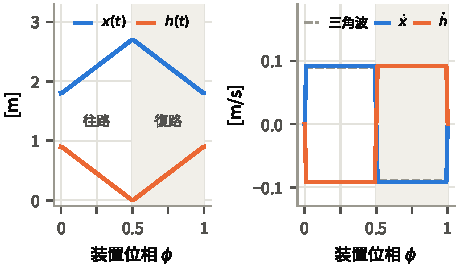
\includegraphics[width=\linewidth]{../results/figs/device_motion.pdf}
\caption{装置運動（$T=20$\,s）．左：先端間距離 $x$ と高低差 $h$．右：装置速度（平滑化と三角波）．}
\label{fig:device}
\end{figure}
\subsection{突起形状と成功条件}
突起は前面から 3\,cm 張り出し，鉛直高さ 5\,cm，その下 15\,cm が本体前面（手首の移動を制限する面），
それより下は開放空間である．先端上縁には手への食い込みを避ける R\,5\,mm の丸みを与えた．
A を両手で把持し胸を A に向けた静止状態から開始し，1 周期 $T$ 以内に離手，B を両手で捕捉して 2.0\,s 保持できれば成功とする．
把持負荷は両手合計の突起反力 $\bm R$ に対し $U=\|\bm R\|/F_{\mathrm{cap}}$，$\Upk=\max_t U$ で表す
（$F_{\mathrm{cap}}$：両手の把持容量，基準値 1300\,N）．努力指標は
\begin{equation}
\Eeff=\frac{1}{t_{\mathrm{ref}}}\int\Bigl\{\frac1{n_j}\sum_j\Bigl(\frac{\tau_j}{\tau_j^{\mathrm{cap}}}\Bigr)^2+U^2\Bigr\}\,dt
\end{equation}
とする（$t_{\mathrm{ref}}=1$\,s）．

\section{縮約モデルと軌道最適化}
\subsection{平面 5 リンク人体}
前腕＋手，上腕，体幹＋頭部，大腿，下腿の 5 リンク（左右合算）を，de~Leva~\cite{deleva1996} の質量比・重心位置・回転半径から
体重 $m$ と身長 $H$（基準 1.75\,m，全リンク長を $H/1.75$ でスケール）に合わせて構成した．
両手の掛かり線（PIP）を基底座標 $\bm p_h$ とし，$\bm q=(\bm p_h,\theta_1,\dots,\theta_5)$ の運動方程式
$\bm M(\bm q)\ddot{\bm q}+\bm h(\bm q,\dot{\bm q})=\bm B\bm\tau+\bm J^\top\bm R$ を CasADi で記号導出した．
把持中は $\bm p_h$ が装置に従属し，$\bm R$ は拘束力として第 1,2 行から得られる．
肘・肩・股・膝のトルク上限（両側合計 120/160/300/240\,N\,m），関節可動域，関節角速度 10\,rad/s，
指令トルク変化率 $10\tau^{\mathrm{cap}}$/s を課した．
\subsection{相構成と捕捉モデル}
待機（静止把持）→振り（A に拘束）→飛行（自由鎖，内部トルクのみ）→捕捉→保持（B に拘束 2.0\,s）の多相問題とした．
捕捉は掛かり線が B 先端に一致し，手先が把持面へ向かう（$v_{\mathrm{rel},y}\le0$，壁から離れる速度 $\le0.5$\,m/s，
$\|\bm v_{\mathrm{rel}}\|\le4$\,m/s）ときの完全非弾性衝突として扱い，
衝撃力積 $\bm\Lambda$ を $\bm M(\dot{\bm q}^+-\dot{\bm q}^-)=\bm J^\top\bm\Lambda$ から求める．
捕捉負荷は，力積を $\Delta_c=50$\,ms に均した力と捕捉直後の持続張力 $\bm R_H(0)$ の重ね合わせ
\begin{equation}
U_{\mathrm{catch}}=\frac{\dfrac{\|\bm\Lambda\|}{\Delta_c}+\|\bm R_H(0)\|}{F_{\mathrm{cap}}}
\end{equation}
とした．突起反力には片側支持 $R_y\ge0$ と摩擦・引っ掛かり錐（壁から離れる向き $\mu_{\mathrm{out}}=1.0$，
壁へ向かう向き $\mu_{\mathrm{in}}=2.0$）を課し，壁・突起との干渉は各部位の平滑化 max 制約で除いた．
\subsection{目的関数と数値法}
「必要把持容量の最小化」を主目的とし，$J=w_U\Upk+w_E\Eeff$（$w_U=10,w_E=1$）を最小化した．
$\Upk$ は epigraph 変数で，$\Upk\times1300$\,N がその離手位相で成功するために必要な両手容量である．
離散化は圧縮型 Hermite--Simpson（振り 150，飛行 30，保持 60 区間，暗黙力学），求解は IPOPT~\cite{wachter2006}（CasADi~\cite{andersson2019}）である．
初期実装で最適化器が離散化誤差を利用して重心を推進する非物理解を返したため，
飛行中の重心放物線・角運動量保存を許容帯付き制約として追加し，全解を RK4 1\,ms で再積分して一致を監査した
（飛行区間の手先誤差 \verFhand\,mm 以下）．
メッシュを 2 倍にした再解で必要容量は $+1.0\%$，努力は $+0.1\%$ しか変わらない．

\section{3 次元人体環境}
体幹 3・頸 2・肩 3・肘 1・前腕回旋 1・手首 2・股 3・膝 1・足首 2（左右計 31）のヒンジ関節と指開閉 2 チャネルをもつ人体を
MuJoCo~\cite{todorov2012} 上に構成した（質量特性は de~Leva，図~\ref{fig:3d}）．
関節はトルク飽和付き PD サーボ，制御周期 20\,ms，物理刻み 1\,ms である．
把持は MuJoCo の軟らかい点拘束（有限剛性）で実装し，各物理ステップで拘束力を読み出して
片側支持・摩擦錐・容量（掛かり代・疲労に依存）を判定，超過分は粘塑性滑りとして積分し，滑り量 2\,cm または掛かりの喪失で剥離させる．
係合には掛かり線が上面上にあること，掌が壁を向くことを要求し，瞬間的な位置合わせ・無限容量拘束・裏面からの吸着を許さない．
半陰的 Euler 積分は放物運動に $g\,\Delta t/2\approx4.9$\,mm/s の系統誤差をもつため，空中区間は RK4，拘束・接触中は暗黙 Euler に切り替えた．
受入試験（表~\ref{tab:accept}）はすべて自動テストとして同梱した．
\begin{table}[t]
\centering\scriptsize
\caption{3 次元環境の受入試験}
\label{tab:accept}
\begin{tabular}{lll}
\toprule
検査 & 目標 & 結果 \\
\midrule
位置・周期 & 端点・周期一致，根元間$=$先端間$+6$\,cm & 一致 \\
自由飛行 & 重心誤差 $\le1$\,mm/s & 0.008\,mm/s \\
角運動量 & 無接触時変化 $\le0.1\%$ & 0.007\% \\
捕捉の力積 & 力積収支残差 $\le1\%$ & 合格 \\
数値収束 & 1 vs 0.5\,ms，10\,ms 平均力差 $\le5\%$ & 1.9\% \\
幾何・拘束 & 下方・裏面からの把持 0 件 & 合格 \\
静的把持 & 両手反力$=mg$ & 誤差 $<0.1\%$ \\
\bottomrule
\end{tabular}
\end{table}

\section{結果}
\subsection{離手位相と必要把持容量}
図~\ref{fig:reqcap} に代表条件（$T\in\{16,19,20,24\}$\,s，$m\in\{60,75\}$\,kg）の離手位相 $\phi_\ell$ 16 点に対する必要両手把持容量を示す
（全体は $T$ \nT\ 点 $\times$ $m$ \nm\ 点 $\times$ 16 位相 $=$ \ncases 条件，収束 \nok 条件）．
位相依存は往路・復路に一つずつ谷をもつ二谷構造で，谷は往路 $\phi_\ell\approx$ \outphimin--\outphimax
（A が中程まで下がり先端間 2.2--2.3\,m）と復路 $\phi_\ell\approx$ \retphimin--\retphimax（同じ幾何で装置速度が反転）にある．
山は $\phi_\ell=0$（先端間 1.80\,m だが落下高さ 0.90\,m）と $\phi_\ell=0.5$（等高だが 2.70\,m）で，
落下高さと水平距離のどちらも捕捉後の張力を押し上げる．山と谷の差は平均 \ptov\,\% である．
最短距離となる $\phi_\ell=0$ で離手すると最良位相より平均 \hTwopenalty\,\%（最大 \hTwopenaltymax\,\%）大きな容量を要し，
最短距離は最小負担ではない．
往路谷と復路谷の差は最大 \hOnediffmax\,\% にとどまり（\ncond 条件中 \nret 条件で復路が最小），
どちらの谷を使うかは装置位相と準備時間で決めてよい程度の差である（表~\ref{tab:best}）．
このため図~\ref{fig:tm} の最良位相は往路谷（$\approx0.25$）と復路谷（$\approx0.7$）の間で条件ごとに入れ替わる．
最適解では振り終盤・捕捉衝撃・捕捉後の振れの 3 箇所で $U$ が同時に $\Upk$ に達しており（図~\ref{fig:traj}），
把持容量が全区間で支配的な制約である．

\begin{figure*}[t]
\centering
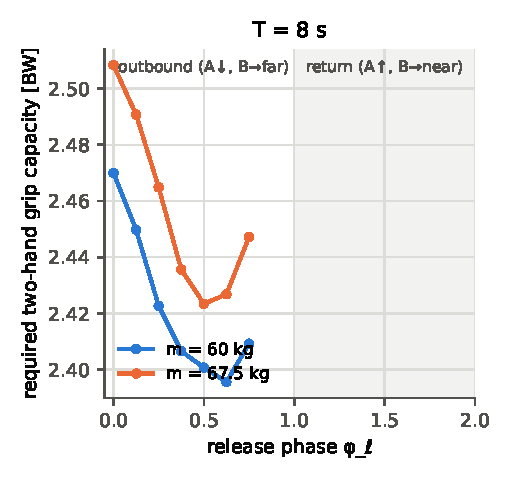
\includegraphics[width=\linewidth]{../results/figs/reqcap_vs_phase.pdf}
\caption{離手位相 $\phi_\ell=(t_\ell \bmod T)/T$ と必要両手把持容量（代表条件）．灰色は復路．
$\times$ は収束解が得られなかった条件（装置折り返し点 $\phi_\ell=0$ 近傍）．}
\label{fig:reqcap}
\end{figure*}
\begin{figure*}[t]
\centering
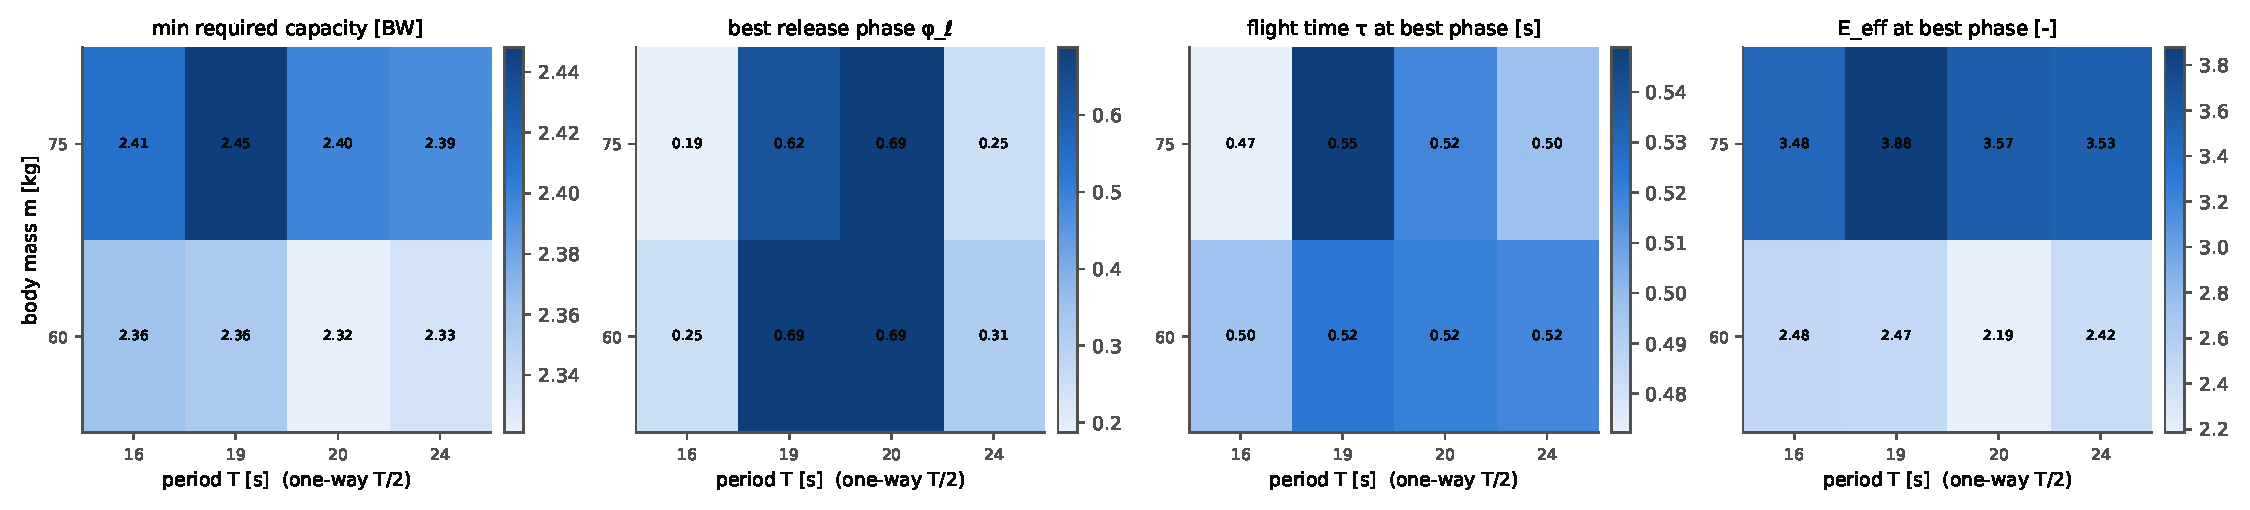
\includegraphics[width=\linewidth]{../results/figs/tm_maps.pdf}
\caption{$T\times m$ マップ（位相について最小化）．左から必要容量 [BW]，最良離手位相，滞空時間，努力指標．}
\label{fig:tm}
\end{figure*}

\begin{table}[t]
\centering\scriptsize
\caption{代表条件の谷の値（必要容量 [BW]，括弧内は位相）と $\phi_\ell=0$ の値，滞空時間．}
\label{tab:best}
\begin{tabular}{rrrrrr}
\toprule
$T$ [s] & $m$ [kg] & 往路谷 & 復路谷 & $\phi_\ell=0$ & $\tau$ [s] \\
\midrule
16 & 60 & 2.36 (0.25) & 2.36 (0.69) & 2.55 & 0.50 \\
16 & 75 & 2.41 (0.19) & 2.42 (0.75) & 2.65 & 0.47 \\
19 & 60 & 2.37 (0.31) & 2.36 (0.69) & 2.55 & 0.52 \\
19 & 75 & 2.45 (0.31) & 2.45 (0.62) & 2.65 & 0.55 \\
20 & 60 & 2.37 (0.25) & 2.32 (0.69) & 2.48 & 0.52 \\
20 & 75 & 2.41 (0.19) & 2.40 (0.69) & 2.58 & 0.52 \\
24 & 60 & 2.33 (0.31) & 2.34 (0.69) & 2.55 & 0.52 \\
24 & 75 & 2.39 (0.25) & 2.41 (0.62) & 2.56 & 0.50 \\
\bottomrule
\end{tabular}

\end{table}

\subsection{$T$--$m$ マップと体格}
図~\ref{fig:tm} に，各 $(T,m)$ で位相について最小化した必要容量・最良位相・滞空時間・努力を示す
（$T$：\Tmin--\Tmax\,s，$m$：\mmin--\mmax\,kg）．
最小必要容量は \bestcapmin--\bestcapmax\,BW で，$m$ に対して体重比でも増加する（60\,kg で \capsixty，75\,kg で \capseventyfive\,BW）．
これは関節トルク上限を絶対値で固定したためで，体重の効果を能力の比例則で打ち消さない設計の帰結である．
$T$ の効きは小さい．滞空 \taumin--\taumax\,s の間に装置が動く距離は数 cm にすぎないからである．
身長 $H\in[1.60,1.85]$\,m と腕長比を変えた体格掃引（$T=20$\,s，$m=66$\,kg，能力は絶対値固定）を図~\ref{fig:build}・表~\ref{tab:build} に示す．
身長の効果は体重と同程度に大きく，最小必要容量は $H=1.60$\,m の \capHonesixty\,BW から $H=1.85$\,m の \capHoneeightyfive\,BW へ単調に減る．
腕長比 $\pm5\%$ でも \capAninetyfive\ から \capAonezerofive\,BW と変わる．
長いリーチは先端間の実効距離を縮め，捕捉後の振り子長を延ばして張力を下げるためである．
\IfFileExists{../results/figs/build.pdf}{%
\begin{figure}[t]
\centering
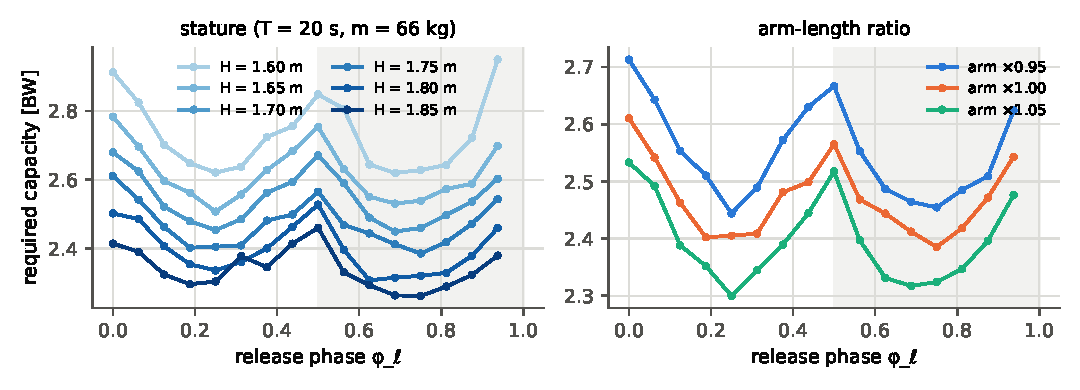
\includegraphics[width=\linewidth]{../results/figs/build.pdf}
\caption{体格掃引：身長 $H$（左）と腕長比（右）に対する必要容量の位相依存．}
\label{fig:build}
\end{figure}}{}
\begin{table}[t]
\centering\scriptsize
\caption{体格掃引の要約（位相について最小化した必要容量）．}
\label{tab:build}
\IfFileExists{tab_build.tex}{\begin{tabular}{rrrrrr}
\toprule
身長 [m] & 腕長比 & 最小 [BW] & 平均 [BW] & 最良 $\phi_\ell$ & $\tau$ [s] \\
\midrule
1.75 & 0.95 & 2.44 & 2.55 & 0.250 & 0.50 \\
1.60 & 1.00 & 2.62 & 2.73 & 0.688 & 0.55 \\
1.65 & 1.00 & 2.51 & 2.62 & 0.250 & 0.50 \\
1.70 & 1.00 & 2.45 & 2.54 & 0.688 & 0.53 \\
1.75 & 1.00 & 2.39 & 2.47 & 0.750 & 0.50 \\
1.80 & 1.00 & 2.31 & 2.40 & 0.625 & 0.54 \\
1.85 & 1.00 & 2.26 & 2.34 & 0.750 & 0.49 \\
1.75 & 1.05 & 2.30 & 2.40 & 0.250 & 0.49 \\
\bottomrule
\end{tabular}
}{（計算中）}
\end{table}

\begin{figure}[t]
\centering
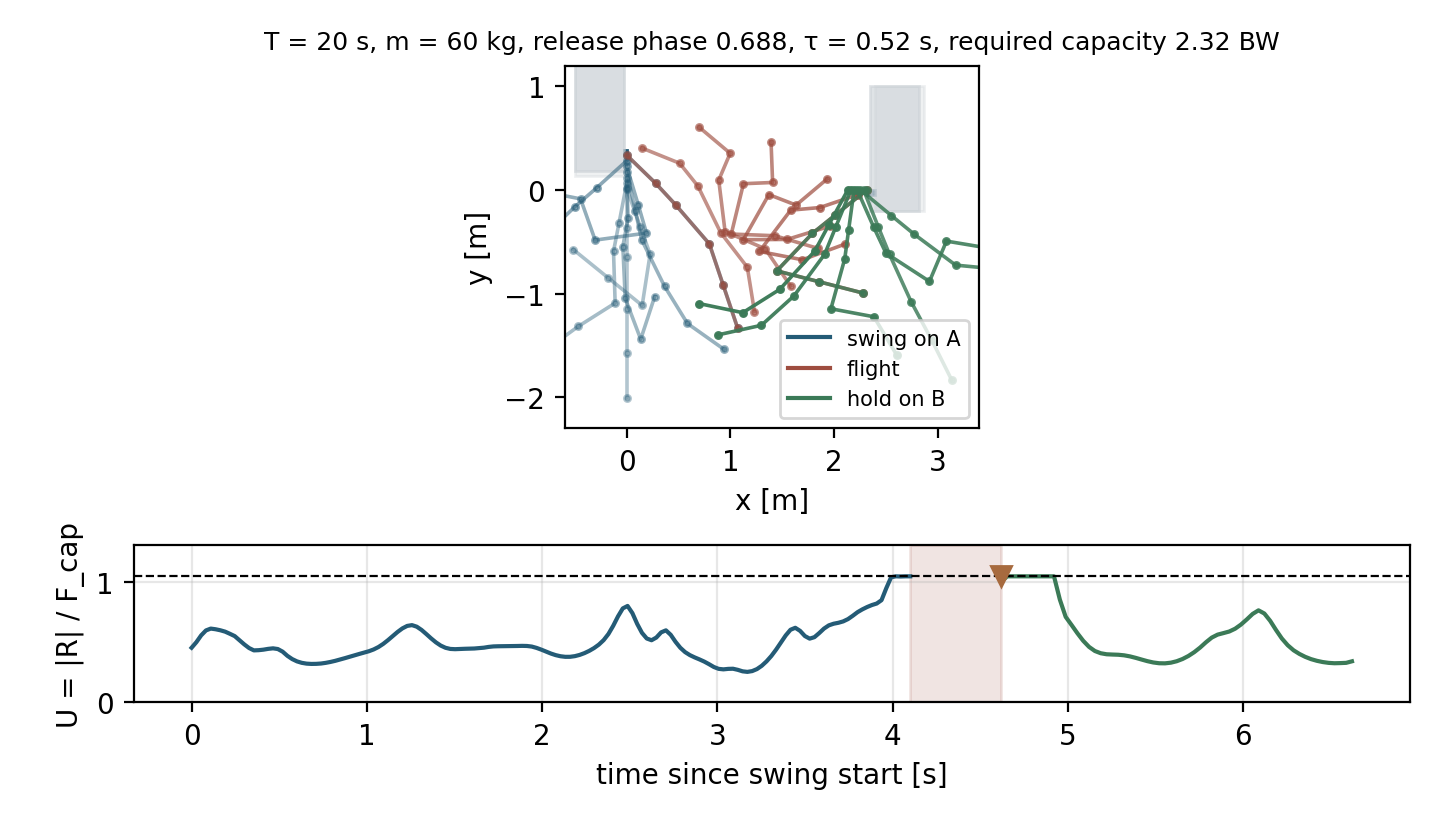
\includegraphics[width=.95\linewidth]{../results/figs/traj_best.png}
\caption{代表解（$T=20$\,s，$m=60$\,kg，最良位相）のスティック図と把持利用率 $U(t)$．
青：A での振り，赤：飛行，緑：B での保持．$\blacktriangledown$ は捕捉負荷，破線は $\Upk$．}
\label{fig:traj}
\end{figure}

\begin{figure}[t]
\centering
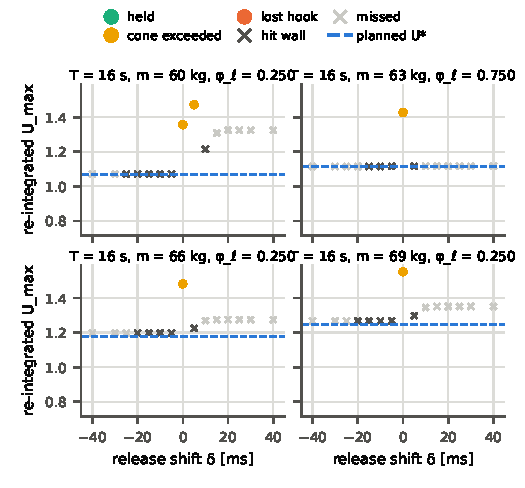
\includegraphics[width=\linewidth]{../results/figs/windows.pdf}
\caption{離手指令のずれ $\delta$ に対する再積分結果（代表 4 条件）．丸は掌が掛かった試行，$\times$ は捕捉失敗．破線は計画値 $U^*$．}
\label{fig:win}
\end{figure}
\subsection{離手タイミングの許容幅}
代表条件の最良解に対し離手指令を $\delta\in[-0.2,0.2]$\,s ずらし，関節は計画軌道への PD 追従
（フィードバック分に 40\,ms の活性化フィルタ，トルク飽和），捕捉は有限剛性（40\,kN/m）の順応把持として 1\,ms RK4 で再積分した
（図~\ref{fig:win}，表~\ref{tab:win}）．
掌が B の上面に掛かる「捕捉窓」は \catchwinmed\,ms（中央値，最大 \catchwinmax\,ms）と極めて狭い．
離手時刻のずれは振りの角速度を通じて射出方向を変え，到達高さを約 1\,cm/ms 動かすためである．
さらに $\delta=0$ でも順応把持で再積分した負荷は計画値 $U^*$ の \loadratio 倍（中央値，最大 \loadratiomax 倍）となり，
摩擦錐の外へ出る瞬間が生じる．剛体衝突を仮定した最適解は制約境界上にあり，実行誤差に対する余裕をもたない．
飛行中の手先補正を持たない開ループ計画では，離手精度 $\pm5$\,ms が要求されることになる．
\begin{table}[t]
\centering\scriptsize
\caption{離手窓の再積分（計画追従モード）．$U$ は $\delta=0$ の再積分値．}
\label{tab:win}
\IfFileExists{tab_windows.tex}{\begin{tabular}{rrrrrrrl}
\toprule
$T$ & $m$ & $\phi_\ell$ & $U^*$ & 捕捉窓 [ms] & $U_{\rm catch}$ & $U_{\rm hold}$ & 再積分結果 \\
\midrule
16 & 60 & 0.250 & 1.07 & 15 & 1.36 & 1.30 & cone exceeded \\
16 & 75 & 0.188 & 1.36 & 10 & 1.72 & 1.72 & cone exceeded \\
19 & 60 & 0.688 & 1.07 & 10 & 1.36 & 1.31 & cone exceeded \\
19 & 75 & 0.625 & 1.39 & 10 & 1.74 & 1.72 & cone exceeded \\
20 & 60 & 0.688 & 1.05 & 10 & 1.35 & 1.30 & cone exceeded \\
20 & 75 & 0.688 & 1.36 & 10 & 1.70 & 1.69 & cone exceeded \\
24 & 60 & 0.312 & 1.06 & 10 & 1.35 & 1.30 & cone exceeded \\
24 & 75 & 0.250 & 1.35 & 10 & 1.70 & 1.69 & cone exceeded \\
\bottomrule
\end{tabular}
}{（計算中）}
\end{table}

\subsection{感度解析}
図~\ref{fig:sens} に $T=20$\,s，$m=60$\,kg，5 位相での一因子感度を示す．
壁から離れる向きの摩擦・引掛り係数 $\mu_{\rm out}$ を 0.6 に下げると必要容量は約 10\,\%，
関節能力を 30\,\% 下げると約 7\,\% 増え，折り返し時間 $\epsilon$，捕捉均し時間 $\Delta_c$，手先相対速度上限の影響は 1--3\,\% にとどまる．
本課題は把持の引っ掛かりと上肢・体幹の能力に律速され，装置側の細部には鈍感である．
\begin{figure}[t]
\centering
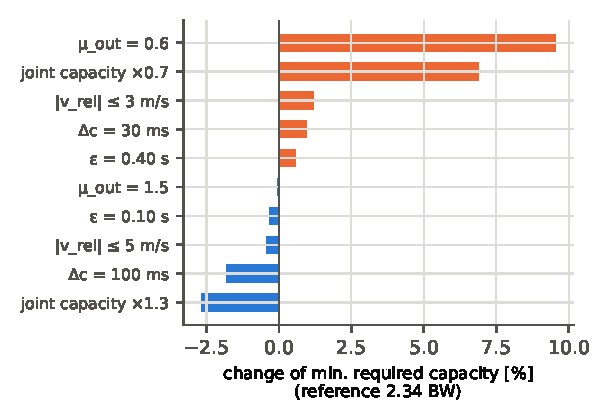
\includegraphics[width=.8\linewidth]{../results/figs/sensitivity.pdf}
\caption{一因子感度：位相について最小化した必要容量の基準値からの変化．}
\label{fig:sens}
\end{figure}

\subsection{3 次元環境での探索}
平面解を矢状面関節へ転写して初期化した CMA-ES 探索（$T=20$\,s，$m=66$\,kg，個体数 32，300 世代，22 並列）では，
胸を B へ向ける再配向は達成されたが（最接近時の胸法線の $x$ 成分 0.95），両手捕捉には至らず
（手先中点と B 先端の最短距離 0.89\,m），振りの途中で把持容量を超えて剥離した（図~\ref{fig:3d}）．
把持容量を緩和した条件から段階的に戻すカリキュラムと，より長い探索を継続している．
\begin{figure}[t]
\centering
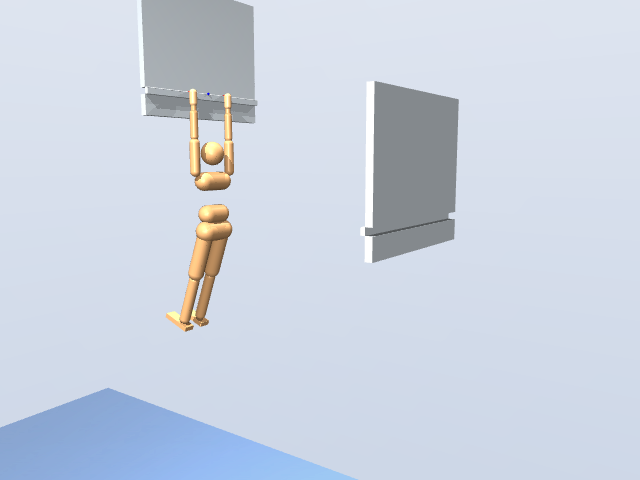
\includegraphics[width=.37\linewidth]{../results/figs/hang3d.png}\hfill
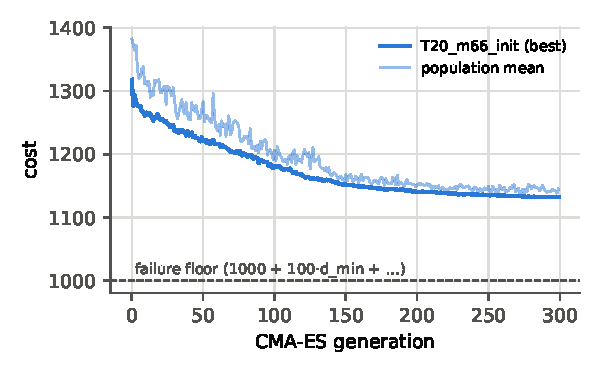
\includegraphics[width=.55\linewidth]{../results/figs/search3d.pdf}
\caption{左：MuJoCo 3 次元環境（A に両手把持した初期状態，右奥が B）．右：CMA-ES 探索のコスト履歴．}
\label{fig:3d}
\end{figure}

\section{議論と限界}
縮約モデルは矢状面のみを扱い，空中での 180 度の向き変え，左右の手の時間差，横ずれを含まない．
把持は両手合算で，容量は体重・体格によらない絶対値である．
捕捉を完全非弾性衝突とし力積を $\Delta_c=50$\,ms に均す近似は，順応把持による再積分で 1.3 倍程度の差を生じた．
これらは「最適解の脆さ」であると同時に，学習段階で閉ループ補正と余裕を含む方策を求めるべき理由である．
必要容量 2.3--2.9\,BW は 3\,cm 縁での両手ぶら下がり能力の上位値に相当し，本課題が把持能力に律速されることを示す．
世界モデル型学習の価値（経験効率）は本稿では未検証であり，同一環境上で SAC・DreamerV3~\cite{hafner2025} と比較する計画である．

\section{まとめ}
クリフディメンションの背面飛び移りを，装置運動・3\,cm 突起・有限把持容量を含む力学課題として定式化し，
決定論的な軌道最適化により離手位相・周期・体重・体格ごとの必要把持容量と離手許容幅を求めた．
往路と復路に一つずつある谷のどちらかで離手すべきこと，最短距離の離手は最小負荷でないこと，
開ループ計画では $\pm5$\,ms の離手精度が要ることを示した．
併せて 33 自由度の 3 次元環境と有限容量把持モデルを検証済みの形で公開し，学習法比較の共通基盤とした．
コードと結果は \url{https://github.com/omotes24/CliffDimension} にある．

\begin{thebibliography}{9}
\bibitem{janner2019} M. Janner, J. Fu, M. Zhang, and S. Levine, ``When to trust your model: Model-based policy optimization,'' Proc. NeurIPS, 2019.
\bibitem{haarnoja2018} T. Haarnoja, A. Zhou, P. Abbeel, and S. Levine, ``Soft actor-critic,'' Proc. ICML, 2018.
\bibitem{deleva1996} P. de Leva, ``Adjustments to Zatsiorsky-Seluyanov's segment inertia parameters,'' J. Biomech., vol.~29, no.~9, pp.~1223--1230, 1996.
\bibitem{wachter2006} A. W\"achter and L. T. Biegler, ``On the implementation of an interior-point filter line-search algorithm for large-scale nonlinear programming,'' Math. Program., vol.~106, pp.~25--57, 2006.
\bibitem{andersson2019} J. A. E. Andersson et al., ``CasADi: a software framework for nonlinear optimization and optimal control,'' Math. Program. Comput., vol.~11, pp.~1--36, 2019.
\bibitem{todorov2012} E. Todorov, T. Erez, and Y. Tassa, ``MuJoCo: A physics engine for model-based control,'' Proc. IROS, 2012.
\bibitem{hafner2025} D. Hafner, J. Pasukonis, J. Ba, and T. Lillicrap, ``Mastering diverse control tasks through world models,'' Nature, vol.~640, pp.~647--653, 2025.
\end{thebibliography}
\end{document}
